%documentclass [12pt]{article}
\documentclass[12pt, oneside]{article}
\usepackage{setspace} % for double-spacing.
\usepackage[top=2.54cm, bottom=2.54cm, left=2.54cm, right=2.54cm]{geometry}	 %
\usepackage{url}
\usepackage{mathptmx}% http://ctan.org/pkg/mathptmx
\usepackage{xifthen}%
%\doublespacing
\usepackage{lipsum}
\usepackage{breakurl}
\usepackage[breaklinks]{hyperref}
\usepackage{tocloft}
\usepackage{color}
\usepackage{array}
\usepackage{stfloats}
\usepackage[pdftex]{graphicx}
\usepackage{subcaption}
\usepackage[export]{adjustbox}
\usepackage{multirow}
\usepackage{url}
\usepackage{changepage}
\usepackage{floatrow}
\usepackage{titlesec}
\usepackage{chngcntr}
\usepackage{fancyhdr}
% -- Define code snippet configuration
\usepackage{listings}
\usepackage{color}
\usepackage{floatrow}

\usepackage{listings}
\usepackage{color}

\definecolor{dkgreen}{rgb}{0,0.6,0}
\definecolor{gray}{rgb}{0.5,0.5,0.5}
\definecolor{mauve}{rgb}{0.58,0,0.82}

\lstset{frame=tb,
  language=Java,
  aboveskip=3mm,
  belowskip=3mm,
  showstringspaces=false,
  columns=flexible,
  basicstyle={\small\ttfamily},
  numbers=none,
  numberstyle=\tiny\color{gray},
  keywordstyle=\color{blue},
  commentstyle=\color{dkgreen},
  stringstyle=\color{mauve},
  breaklines=true,
  breakatwhitespace=true,
  tabsize=3
}

\title{Using IBM's Tonality Analysis of Language and Geolocated Tweets to Map Emotional Intensity.
\\\medskip}
\author{Isaac Callison (ic2d@mtmail.mtsu.edu)\\Middle Tennessee State University}

\begin{document}
\maketitle
\nocite{*}
\newpage{}


\renewenvironment{abstract}
 {\small
  \begin{center}
  \bfseries \abstractname\vspace{-.5em}\vspace{0pt}
  \end{center}
  \list{}{
    \setlength{\leftmargin}{.8cm}%
    \setlength{\rightmargin}{\leftmargin}%
  }%
  \item\relax}
 {\endlist}

\begin{abstract}
The corpus of social-media data as a whole is growing at an exponential rate
and extraction of useful information from that data is exploding.
Big Data focused companies and organizations are competing at a furious rate to
glean advantages from ever expanding datasets. One such voluminous and
continuously expanding dataset are tweets from the social-media giant Twitter.
Tweets from various regions were collected in real-time using Tweepy.
Geolocation was obtained through location parsing and geocoding. Using IBM's
tone analyzer, the emotional nature of these tweets was analyzed and the
predominant emotion and intensity was extracted. The results were mapped onto a
Google Heatmap.
\end{abstract}

\section{Introduction}
\paragraph{}
There is a convergence of powerful technologies that allow for near-
instantaneous notification of current events using available from
social media platforms. In some cases these technology tools are the medium by
which revolutions are fomented and driven\cite{arab}. This is the era of "Big
Data" that measures in the realm of zettabytes, the unspoken hypothesis is that
one can presume a postive correlation between the growing data and the
usefulness that can be extracted from said data\cite{villars2011}.

One social media platform for which, at least the possibility of obtaining
relevant data is present, is Twitter. This reality is not lost
on Twitter. In fact, part of Twitter's business model is selling user data
through premium API's\footnote{https://developer.twitter.com/en/premium-apis}.

The goal of this project was to gather and analyze tweets for emotive tonality,
then display this on a "heatmap"\footnote{A heatmap is a graphical
representation of data that uses a system of color-coding to represent
different values.} of emotive intensity for a specific
region. To this end three separate technologies were utilized. For this
project  these technologies were interdependent. First, using Twitter's
developer API, geolocated tweets were collected from a specific region, then
pre-processed to extract latitude, longitude and text. Secondly, using IBM's
Watson and natural language processing capabilities, the tweets were assesed
for emotive tonality. Finally, a Google map was
displayed with a heatmap layer graphing the intensity of these emotions.

In a perfect world with enough data coming in of the type referenced above, a
real-time map of the emotional state of a town or city could be analyzed. The
reality fell far short of what was envisioned and the the successes and
shortcomings will be documented herein.


\section{Background}
\paragraph{}
As stated above, there were several interdependent moving parts with this
project. With regards to development environment, a Jupyter Notebook was used
for this project to pull in modules, access API's, and make GET and POST
requests to those APIs.

The proiject's datasets for the natural language processing came from Twitter.
The Twitter API allows for the triangulation of tweets provided certain
data\cite{TwitterGeo}. In general, tweets have a great deal of metadata bundled
into their JSON objects.

A key part of this project was the the triangulation data associated with
tweets. This is certainly not the first project to leverage geotagged tweets
for Big Data. Projects have used it for situational awareness in
diasters\cite{verma2011} and for tracking tourism globally \cite{tourism2013},
to name just two. Papers in the recent past have created high-quality mappings
for geo-tagged tourist tweets\cite{tourist2018}. However, the ability to
extract out latitude and longitude
from a tweet, which was previously available, was culled in June of
2019\footnote{The author was not aware of this change when launching this
project. Please see: https://www.engadget.com/2019-06-19-twitter-removes-
precise-geo-tagging.html}. In response, other methods were used to triangulage
tweets.

Using developer authentication, and a GET request with certain location
parameters, one can obtain a list of current tweets within a search radius in
JSON format. A great deal of data is returned in this format, but from
these tweets one can glean a myriad of information, including up until
recently, the latitude and longitude of the tweet.

The second part of this project was natural language processing with IBM's
Watson using tonality analysis. IBM has a cloud computing program with various
machine learning capabilities\cite{IBM}, one of which is tonality analysis. The
natural language tonality processing that Watson offers can, among other
things, extract emotion from a corpus. In this specific case, a variety of
emotional states could be extracted including: fear, joy, analytical,
confident, sadness, tentative, and anger\footnote{These are the exact tags
assigned to individual sentences.}. Further, the intensity of a specific
emotion can derived at the sentence and document level.

As a graphical representation of the data collected, a heatmap was used. A
heatmap overlay is a feature offered by Google Maps. It can create a
visualization to depict the magnitude variation of data at a range of
latitudinal and longitudinal points. A heatmap is very usefule when you have a
great deal of data points of varying magnitude and their geographic position.
One type of dataset that lends itself well to such graphical representation is
eathquake data\footnote{An eathquake
dataset is included in the gmaps package and is used for illustration and
tutorials}. When the Heatmap Layer is enabled, a colored overlay will appear on
top of the map. By default, areas of higher intensity or magnitude will be
colored red, and areas of lower intensity will appear green\cite{Google}.

\section{Research Method}
\paragraph{}
The consoles and APIs of Twitter, IBM's Watson, and Google were
accessed. The three aformentioned services required developer accounts to be
used. Twitter's API required an application and pre-approval. These
credentials were secured and inserted directly into the code for ease.
Initially, separate Notebook's were used to test the various API's before
integration into the main Notebook.These accounts were free to use, up to a
point. After some extensive testing with IBM's Watson an
upgraded account had to be setup to continue.

All work was done on a Linux desktop environment. Code was written in Python
3. Anaconda was used to launch the Jupyter environment. Postman, a REST API testing software was used to experiment with Twitter's
API\cite{Postman} before integrating Tweepy's tweet streaming code into the
main Notebook.

Using the Python Tweepy\footnote{https://www.tweepy.org/} module GET requests
were made to stream a set number of
tweets for analysis. The original plan was to extract the latitude and
longitude directly from the tweet, and of course
the text of the tweet itself. Because Twitter no longer provides the latitude
and longitude of tweets a workaround was required. Fortunately, some of the
tweets also had embedded address location. An open source API called
Nominatum\footnote{https://nominatim.org/} was used to reverse geocode
addresses which were still embedded in tweet data.

Using the modified method, the Tweets pulled in by the Notebook and subjected
to significant pre-processing. Of the multitude of tweets that were pulled in,
only a fraction made it through the several filters set up. Tweepy allows for
filtering by a bounding-box defined by four coordinates delineated by
two latitude points and two longitude points. Several of these regions were set
into variables for use including the rough bounding-boxes of New York
City, Nashville, Hawaii, and The United States of America. In addition, Tweets
less than 45 characters in length were excluded as it was presumed no
meaningful emotional context could be derived from a shorter tweet.
Tweets were excluded if the tweet meta-data indicated it was in any language
other than English to avoid confusing the Tone Analzer. Tweets with incomplete
addreses were filtered out as well as the geocoder would only work with
complete addresses. Initially retweets were excluded, then allowed on the
theory that a retweet would mirror the retweeter's mood and allow for more data
collection. Finally, a regex expression was used to strip out extraneous
symbols from the tweet.

The cleaned text from the obtained tweets were passed into Watson for tonality
processing. IBM provides a Watson Software Development Kit for integration into
Python and Jupyter\footnote{https://cloud.ibm.com/docs/services/watson?topic=watson-using-sdks}.

Display a heatmap of emotion in a certain region based on the intensity
of the selected emotional state. A Google
Map will display a heatmap layer with the attendant emotion and intensity. For
instance, in areas of a region where the tweets have low sadness, green shading
will predominate, changing to red as the intensity of that emotion increases


\section{Results and Analysis}
\paragraph{}
A description of the results gleaned through this process is best addressed
though an analysis of each API service. As the project progressed, three
interdependent API services became four interdependent APIs. Initially
considered
were, Twitter, IBM Watson, and Google. Once it became clear that latitude and
longitude information could not be pulled directly from twitter data, a fourth
API, Nominatum was brought into the fray for geocoding.

Pulling tweets using Tweepy and Twitter's API proved to be fairly straight-
forward once the authentication code was properly set up. As previously
lamented, the fine-grain location data of each tweet was removed
by Twitter in mid-2019. As a result, tweets could be pulled from a specific
region through Tweepy, but the exact latitude and longitude of that
tweet was not discernable. What was initially envisioned was a fine-grain heatmap showing data across a city, but this was not to be the result.

There were two crippling realities grappled with concerning Twitter's API. The
first is that though thousands of tweets could be pulled in a matter of
seconds, after filtering by length, language, and geocoding through Nominatum,
attrition was extremely high. A flood of tweets was turned into a trickle
whereby a usable tweet would come in every few seconds. The second issue was
rate-limiting \footnote{https://developer.twitter.com/en/docs/basics/rate-
limiting}. With all the filters in place, less than 300 tweets could be pulled
in during a half-hour period. At that point an error would be returned by the
twitter API. This exception was caught in the code and an exponential backoff
was implemented to attempt the stream again at a later point. By relaxing a few
of the filters, including allowing retweets, the number of tweets available
before rate-limiting kicked in was increased to around 1200. However, it could
take easily an hour to pull in that many tweets which defeated the "real-time"
nature of the project. The usable tweets and their geocodes were loaded into a
Pandas dataframe object.

Watson's Tone Analysis worked with very few caveats. The free account was
limited to 2500 API calls per month. As such a premium account was setup to
continue its use. The tone analysis worked well at classification, but the
documentation gave little guidance on how to parse the data returned and
offered no function calls that could be used to pull out specific data objects.

The cumbersome JSON data object returned was converted to Python nested
dictionary objects and parsed. Often more than one emotive quality was returned
but sometimes the API could not determine the emotive nature of the tweet and
would return null. The tweet was classified by the predominant emotional
quality returned. The aforementioned Pandas dataframe was amended to include
these attributes and the magnitude of these attributes as returned by the tone
analyzer.

\begin{figure}[H]
\centering
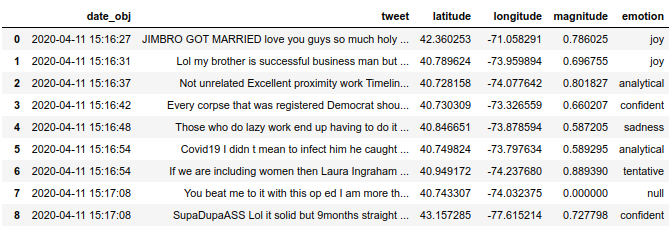
\includegraphics[width=0.7\textwidth]{dataframe}
  \caption{Selected rows of Pandas Datframe}
\end{figure}

A Google API key was used to configure gmaps and display a heatmap overlay. Of
all the API's this one, once setup\footnote{See the environment setup in the
appendix.}, worked the most reliably. The heatmap was populated using the
dataframe. However, to clarify the type of emotion that was represented, only
those rows that had the selected emotion were displayed. For instance, the
following code could be used to load all rows with the emotion "joy" for later
display:
\begin{figure}[H]
\begin{lstlisting}
// Heatmap Notebook
// Defining a variable df_joy from the df object wherein all rows selected have
//"joy" as the requsite emotion

df_joy = df.loc[df['emotion'] == 'joy']
\end{lstlisting}
\caption{Example Starting File for esp8266 devices.}\
\label{fig:code}
\end{figure}

Of one-thousand usable tweets pulled from the New York City region, and
displayed by the variable emotion, this result is produced:

\begin{figure}[H]
\centering
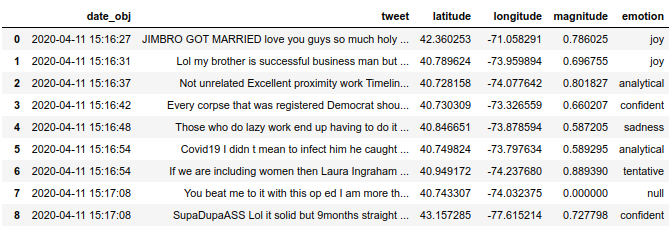
\includegraphics[width=0.7\textwidth]{dataframe}
  \caption{Selected rows of Pandas Datframe}
\end{figure}

Nominatum was the last API referenced above. It had the minor, yet crucial task
of geocoding the addresses pulled from usable tweets. In fact, whether a
tweet had a fairly complete address for geocoding puroposes was one of the
criteria for whether or not a tweet was usable. While this open-source API
provided a work-around for the lack of Twitter embedded coordinates, it was not
always completely accurate. If a partial address was enough to provide
coordinates, Nominatum was used.


\section{Conclusion and Future Work}
We live in an age of ever expanding data, "Big Data" as it is often called. As
the volume of this data increases, data scientists will seek to harness this
information through new technologies, for better or worse. In
this project, an attempt was made to sift a vast amount of Twitter data in
real-time to graph the emotional state of particular regions. Unfortunately,
the particular type of implementation envisioned was ultimately unsuccessful.
Graphing the emotional intensity of differing regions based on twitter content
proved intractable due to miniscule amount of usable geo-taggable tweets that
could actually be assessed for emotional content.

\newpage{}

\bibliographystyle{myplain}
%\bibliographystyle{IEEEannot}
\bibliography{annot}

\newpage{}
\appendix{}
\section{Coding Environment}
All code was run on Ubuntu 18.04 LTS. Anaconda was installed and Jupyter
Notebooks were utilized. All code was written in Python 3. There was some
difficulty in getting Google Maps to display in JupyterLab. Several modules
were required to run the various APIs utilized in this project. The following process was used to install Anaconda and the modules used:

\begin{figure}[H]
\begin{lstlisting}


// From a bash command prompt:
curl -O https://repo.anaconda.com/archive/Anaconda3-5.2.0-Linux-x86_64.sh
bash Anaconda3-5.2.0-Linux-x86_64.sh


// After installation of Anaconda, these modules should be installed:
pip install ibm_watson
pip install tweepy
pip install geopy

// For gmaps:
jupyter nbextension enable --py --sys-prefix widgetsnbextension
pip install gmaps
jupyter nbextension enable --py --sys-prefix gmaps

\end{lstlisting}
\caption{Anaconda \& Module Setup}\
\label{fig:code}
\end{figure}

\end{document}
